\chapter{Architektura odbiornika}

\section{Wstęp}
Wszechstronność systemu była jednym z wymogów projektowych architektury odbiornika. 
Dostosowanie do różnych rodzajów modulacji, pasm częstotliwości i mocy odbieranego sygnału nie powinno powodować zmian w konfiguracji sprzętowej.
Jednostką zarządzającą działaniem odbiornika będzie komputer PC.
Również na nim miejsce będzie miała eliminacja zakłóceń, zatem moduł radiowy powinien posiadać interfejs o wysokiej przepustowości.

\section{Radio definiowane programowo}
Odpowiedzią na stawiane wymagania jest Radio Definiowane Programowo, w skrócie SDR od ang. \textit{Software Defined Radio}.
Dzięki zastosowaniu cyfrowych mieszaczy i filtrów urządzenie może zostać przeprogramowane do celów, których nikt nie przewidział na etapie projektowania systemu telekomunikacyjnego.
Stanowi pewne zabezpieczenie na wypadek zmiany koncepcji lub pojawienia się nowego standardu, ponieważ nie wymaga ingerencji w infastrukturę sprzętową, której modernizacja może przewyższać koszt SDR.
Radio programowalne pozwala na szybkie prototypowanie przy użyciu środowisk dostępnych na różnych systemach operacyjnych. 
Programy takie jak Matlab, Simulink, LabView lub wykorzystywany w tym projeckie GnuRadio, oferują łatwość użytkowania bez specjalistycznej wiedzy z zakresu archiektury procesorów sygnałowych. \cite{ImplementingSDR:92304} 

\section{USRP}
\subsection{Architektura}
Architektura SDR przedstawiona na Rysunku \ref{usrp_architecture} jest wspólna dla wszytkich produktów z rodziny USRP. Po przejściu przez wzmacniacz, sygnał analogowy trafia na demodulator kwadraturowy, który rozdziela jego składowe $I$ i $Q$. 
Widmo sygnałów w.cz. przeniesione zostaje do pasma podstawowego (BB) lub pośredniego (IF). 
Wtedy następuje konwersja analogowo- cyfrowa. 
USRP posiada po dwa przetworniki ADC na każdej lini TX/RX.
Układ FPGA realizuje funkcję konwertera DDC (ang. \textit{Digital Down Converter}), który ogranicza liczbę próbek wyprodukowanych przez ADC, zachowując informację niesioną przez sygnał.
Mniejsza przepływność bitowa pozwala na efektywne przesyłanie danych z USRP do komputera w celu dalszego przetwarzania. \cite{usrp_bw}

\begin{figure}
\centering
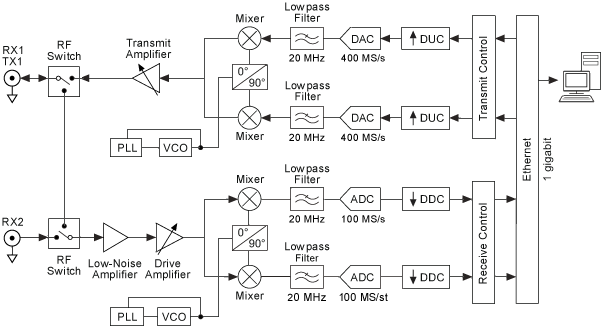
\includegraphics[scale=0.8]{ch4_usrp_architecture.png}
\caption{Architektura USRP}
\label{usrp_architecture}
\end{figure}

\subsection{Wybór właściwego USRP}
USRP występuje w wielu modelach, 

Pytania na które należało odpowiedzieć
\begin{enumerate}
\item Jaki jest wymagany zakres częstotliwości pracy odbiornika?
\item Jakiej szerokości pasmo odbiornik powinien odbierać?
\item Czy odbiornik będzie jednostką autonomiczną czy współpracującą z hostem (PC)?
\item Czy wymagana jest komunikacja dwukierunkowa (full duplex)?
\item Czy obsługiwany będzie tryb MIMO?
\end{enumerate}

\paragraph{Pasmo}
Istnieją trzy typy pasma:
\begin{enumerate}
\item analogowe - to szerokość użytecznego (3dB) pasma pomiędzy wejściem w.cz., a interfejsem radiowym częstotliwości pośredniej lub podstawowej. Zazwyczaj ograniczany przez filtry pasmowe na płycie rozszerzeń.
\item przetwarzania układu FPGA- to częstotliwość próbkowania przetworników ADC na płycie bazowej. Jest to maksymalna hipotetyczna szerokość pasma dla USRP.
\item hosta - Interfejs do wymiany strumieni danych pomiedzy USRP a hostem również posiada swoje ograniczenia. Przepustowość zależy od rodzaju transmisji (simplex lub duplex) oraz liczby bitów przypadającej na jedną próbkę (8 lub 16 bitów). 
\end{enumerate}

Za pasmo całego systemu przyjmuje się najwęższe z wymienionych powyżej. \cite{usrp_bw}
 
\paragraph{Interfejs} Dane pomiędzy radiem a hostem można przesyłać przez jeden spośród kilku interfejsów do wyboru. Najbardziej popularne to:

\begin{enumerate}
\item USB 3.0 - posiada przepustowość ok. 61.44 MS/s.
Ze względu na to, że USB wykorzystuje wspólną linię do nadawania i odbierania danych zezwala jedynie na połączenie half duplex.
\item Gigabit Ethernet - przepustowość 25 MS/s w trybie full duplex. Dodatkową zaletą jest możliwość włączenia urządzenia do sieci i komunikowania się na dużą odległość.
\end{enumerate}

\begin{table}[t]
\caption{Zestawienie parametrów USRP współpracujących z PC}
\label{usrp_table}
\centering
\begin{tabular}{|l|l|l|l|l|}
\hline
Model & Interfejs & Host BW (MS/s) & ADC (MS/s) & MIMO \\
\hline
N210 & GigE & 50@16b 100@8b  & 100 & Tak \\
\hline
N200 & GigE & 50@16b 100@8b  & 100 & Tak \\
\hline
B210 & USB 3.0 & 61.44 & 61.44 & Tak \\
\hline
B210 & USB 3.0 & 61.44 & 61.44 & Nie \\
\hline
\end{tabular}
\end{table}


Odpowiadając na pytania 1 i 2: Większość popularnych naziemnych systemów telekomunikacyjnych pracuje w paśmie do 5 GHz, zatem nie ma potrzeby przekraczania tej częstotliwości. Górną granicę szerokości kanału dla pojedynczej technologii stanowi WiFi z maksymalną szerokością 40 MHz. \cite{802.11}

Odnosząc się do pytania 3. - Ze względu na łatwość prototypowania i dostępność komputera PC, radio będzie współpracowało z komputerem stacjonarnym. Komunikacja full duplex nie jest konieczna, co jest odpowiedzią na pyt. 4., lecz mobilność komputera jest ograniczona na tyle, że konieczne będzie zarządzanie zdalne poprzez interfejs Gigabit Ethernet. Projekt nie przewiduje również pracy w trybie MIMO (pyt. 5)

Tabela \ref{usrp_table} przedstawia krytyczne z punktu widzenia projektu parametry radia. Jeżeli ograniczymy wybór do urządzenia z interfejsem GigE, pozostanie rozstrzygnąć pomiędzy modelem N210 a N200. Różnią się one jedynie ilością bramek w układzie FPGA, których to N210 ma więcej. Wykonanie projektu nie przewiduje przeprogramowania tego układu, zatem rozszerzanie FPGA nie jest konieczne. Wybrany został model N200 (Rysunek \ref{n200}).

\begin{figure}[t]
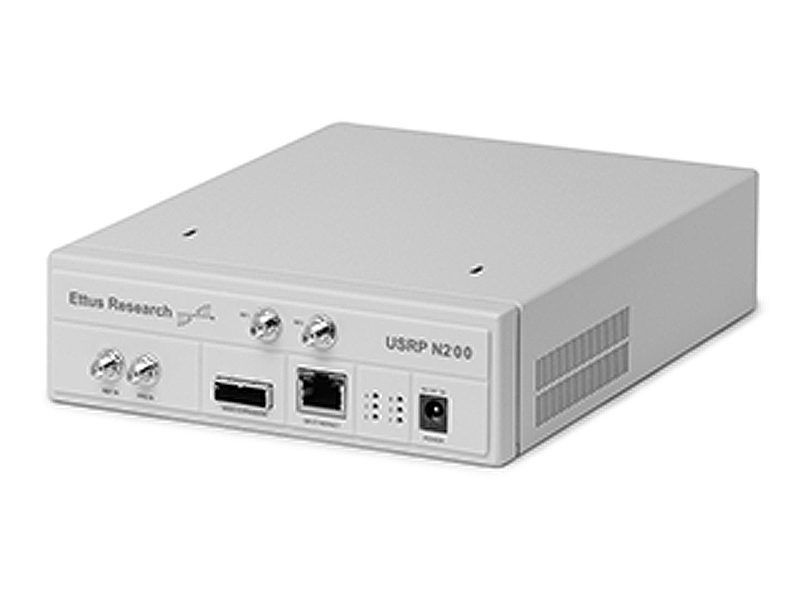
\includegraphics[scale=1]{ch_4n200}
\centering
\caption[Model USRP N200 w obudowie.; Źródło: \textit{https://www.ettus.com/product/details/UN200-KIT}]{\tabular[t]{@{}l@{}}Model USRP N200 w obudowie. \\ Źródło: \textit{https://www.ettus.com/product/details/UN200-KIT}\endtabular}
\label{n200}
\end{figure}



        


